\chapter{Manual de usuario}

\bigskip
Presentamos ahora un manual de usuario de las funciones principales de la aplicación.

\bigskip
\textbf{Nota:} Aplicación desplegada en Heroku en la dirección: \\
\href{https://blooming-citadel-54441.herokuapp.com/datareader}{https://blooming-citadel-54441.herokuapp.com/datareader}

\subsection{Pantalla principal, inicio de sesión y registro}

\bigskip
La primera pantalla que encontramos nos da la bienvenida, y si no tenemos la sesión iniciada nos ofrece dos formularios, uno para iniciar sesión y otro para registrarnos como nuevo usuario:


\begin{figure}[!ht]
  \begin{center}
     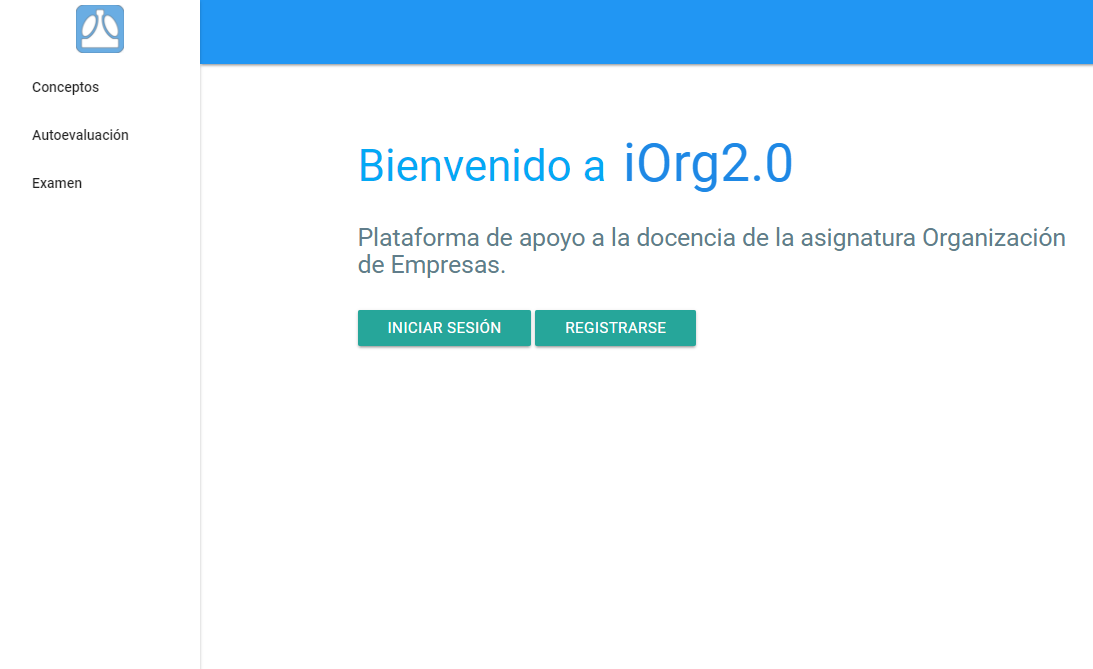
\includegraphics[width=0.8\textwidth]{../images/manual/home.png}
    \caption{Pantalla principal.}
    \label{fig:home}
  \end{center}
\end{figure}

\begin{figure}[!ht]
  \begin{center}
    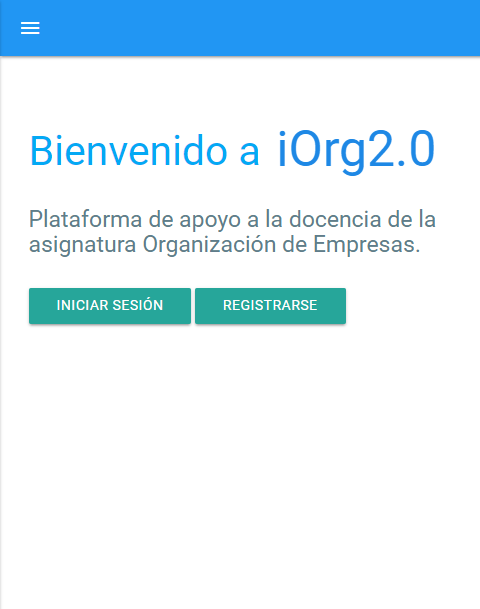
\includegraphics[width=0.6\textwidth]{../images/manual/home_m.png}
    \caption{Pantalla principal versión móvil.}
    \label{fig:home_m}
  \end{center}
\end{figure}



\bigskip
Es necesario iniciar sesión para trabajar con la aplicación, por lo que si intentamos entrar en las secciones del menú lateral seremos redirigidos a la misma pantalla.

\bigskip
Para iniciar sesión seleccionamos el botón ``Iniciar sesión'', si por el contrario no tenemos un usuario necesitaremos registrarnos con el botón ``Registrarse'':


\begin{figure}
 	\centering
    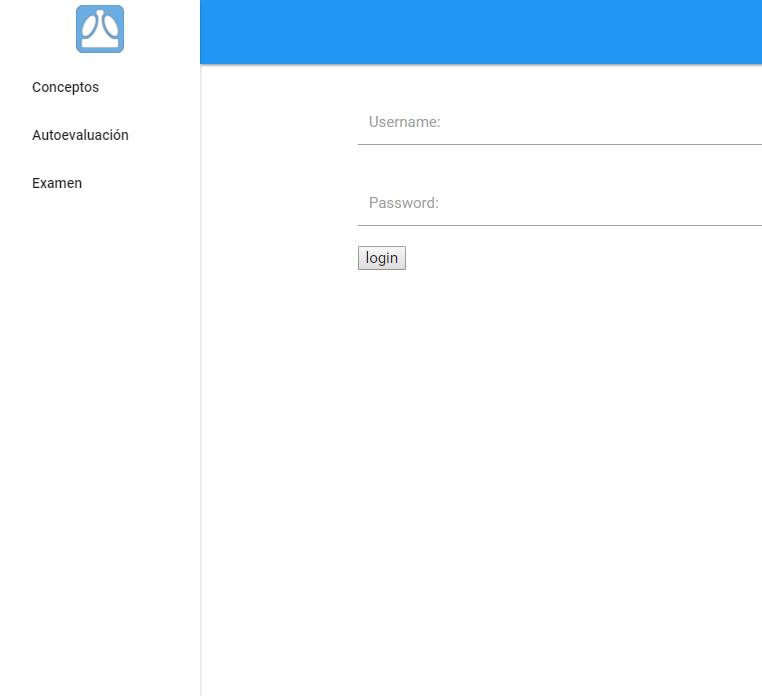
\includegraphics[width=0.6\textwidth]{../images/manual/login.png}
    \caption{Formulario de inicio de sesión.}
	\label{fig:man_login}
	\\
 	\centering
    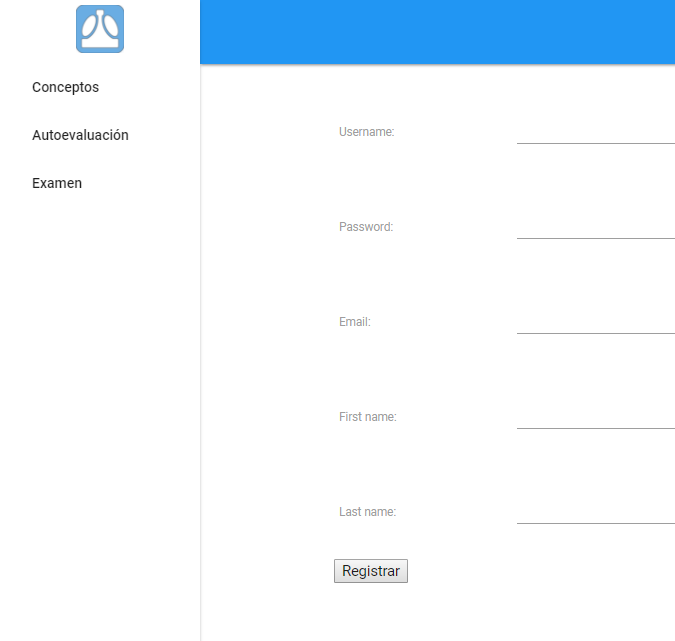
\includegraphics[width=0.6\textwidth]{../images/manual/registrar.png}
    \caption{Formulario de registro de usuario.}
    \label{fig:man_register}
\end{figure}




\newpage

\subsection{Pantalla principal de una sesión iniciada}

\bigskip
Una vez iniciamos sesión, el sistema nos muestra nuestro nombre en la pantalla de bienvenida.
La principal diferentecia que encontramos entre los dos tipos de usuarios (profesor y alumno) es el botón de sitio de administrador en la barra superior.


\begin{figure}[!ht]
  \begin{center}
    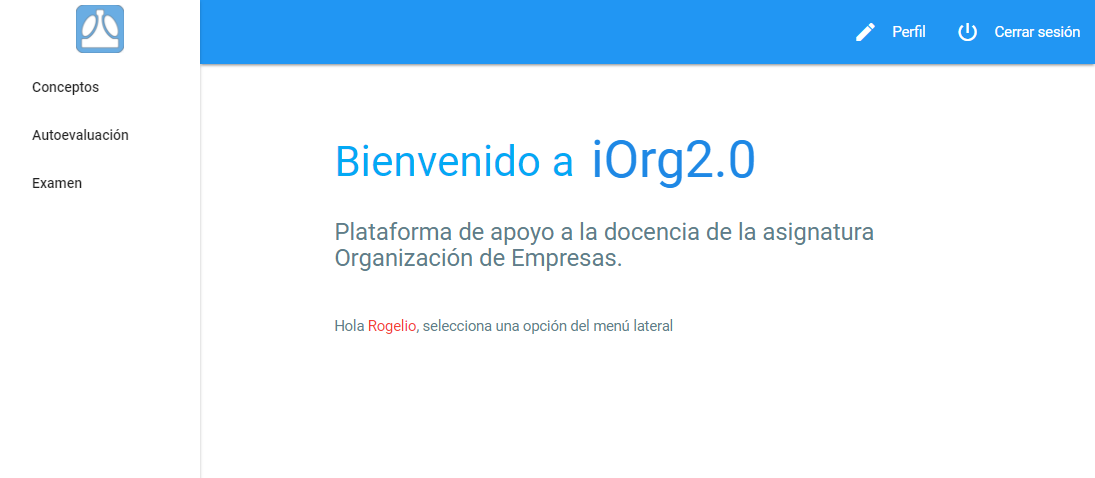
\includegraphics[width=1\textwidth]{../images/manual/home_user_alumno.png}
    \caption{Sesión iniciada como alumno.}
    \label{fig:man_home_user_alumno}
  \end{center}
\end{figure}


\begin{figure}[!ht]
  \begin{center}
    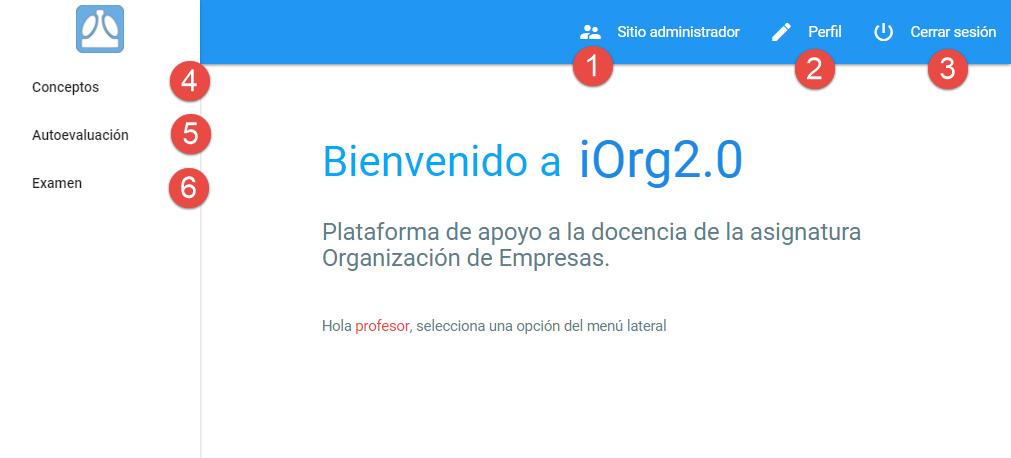
\includegraphics[width=1\textwidth]{../images/manual/home_user.png}
    \caption{Sesión iniciada como profesor.}
    \label{fig:man_home_user}
  \end{center}
\end{figure}


\bigskip
 \begin{itemize}
    \item \textbf{1: Sitio administrador (sólo profesores)} Sección donde podremos actualizar la base de datos de la aplicación consultando la hoja de Google Drive.
    \item \textbf{2: Perfil.} Muestra la información almacenada durante el registro de usuario y  las estadísticas generadas por la aplicación.
    \item \textbf{3: Cerrar sesión.} Desconecta la sesión de usuario.
    \item \textbf{4: Conceptos.} Consultamos una lista de temas que contienen los conceptos básicos de la asignatura.
    \item \textbf{5: Autoevaluación.} Muestra las actividades disponibles en la aplicación.
    \item \textbf{6: Examen} Muestra los tipos de exámenes disponibles para realizar en la aplicación.
 \end{itemize}












\newpage

 \subsection{Conceptos}

 \bigskip
 Una vez pulsamos en esta sección vemos la lista de temas de la asignatura. Al pulsar sobre un tema se despliega apareciendo subtemas, si los hubiese, y los conceptos. Imagen \ref{fig:man_conceptos}.

\bigskip
 \begin{itemize}
    \item \textbf{1: Tema.}
    \item \textbf{2: Subtema.}
    \item \textbf{3: Concepto.}
 \end{itemize}


\begin{figure}[H]
 	\centering
 	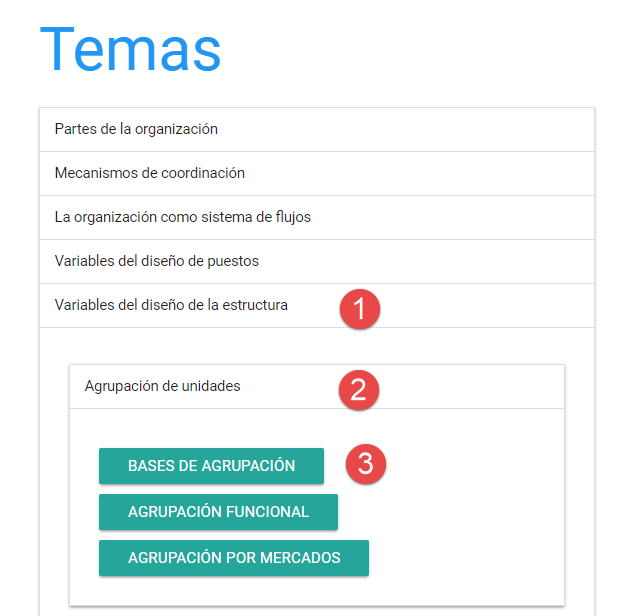
\includegraphics[width=0.8\textwidth]{../images/manual/conceptos.png}
    \caption{Sección conceptos.}
    \label{fig:man_conceptos}
\end{figure}



 \bigskip
 Si hacemos ``click'' sobre uno de los conceptos, aparece una ventana emergente con:

\begin{itemize}
    \item Nombre del concepto.
    \item Definición.
    \item Ejemplo.
    \item Imagen (si la hubiese).
 \end{itemize} 

\bigskip
Lo podemos ver en la siguiente captura \ref{fig:man_concepto_single}.


\begin{figure}[H]
 	\centering
 	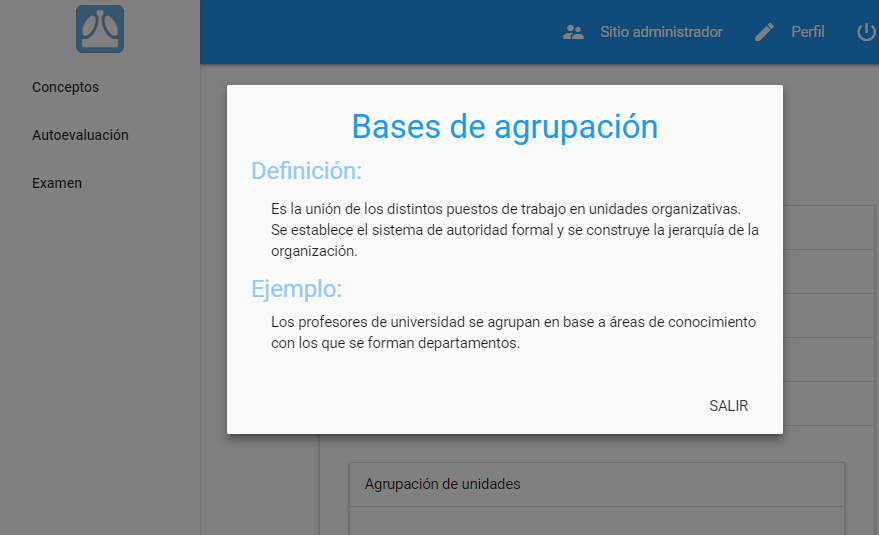
\includegraphics[width=0.8\textwidth]{../images/manual/concepto_single.png}
    \caption{Concepto seleccionado.}
    \label{fig:man_concepto_single}
\end{figure}



\newpage
\subsection{Autoevaluación}

\bigskip
Dentro de la sección de autoevaluación encontramos las secciones de ``Preguntas verdadero y falso'' y ``Preguntas de opción múltiple''. Imagen \ref{fig:man_autoevaluacion}.

\begin{figure}[!H]
 	\centering
 	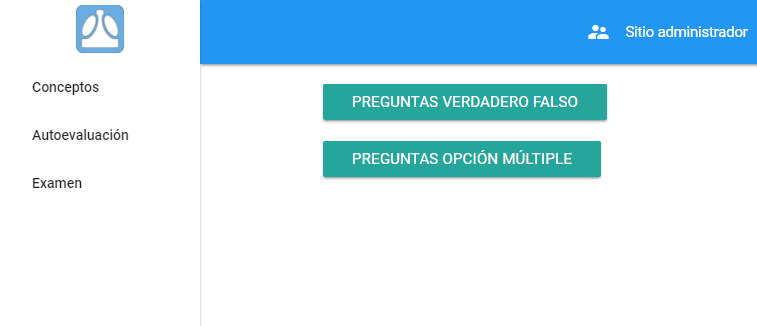
\includegraphics[width=0.8\textwidth]{../images/manual/autoevaluacion.png}
    \caption{Autoevaluación.}
    \label{fig:man_autoevaluacion}
\end{figure}



\bigskip
En ambas secciones encontramos una lista de temas que, al hacer click, el sistema selecciona una pregunta aleatoria de dicho tema y muestra al usuario.


\begin{figure}[!H]
 	\centering
 	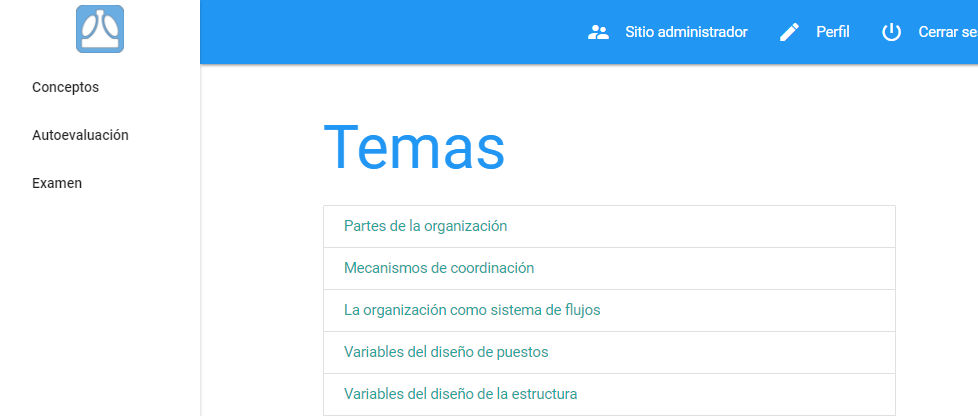
\includegraphics[width=0.7\textwidth]{../images/manual/preguntas.png}
    \caption{Lista de temas para las preguntas.}
    \label{fig:man_preguntas}
\end{figure}


\begin{figure}[!H]
 	\centering
 	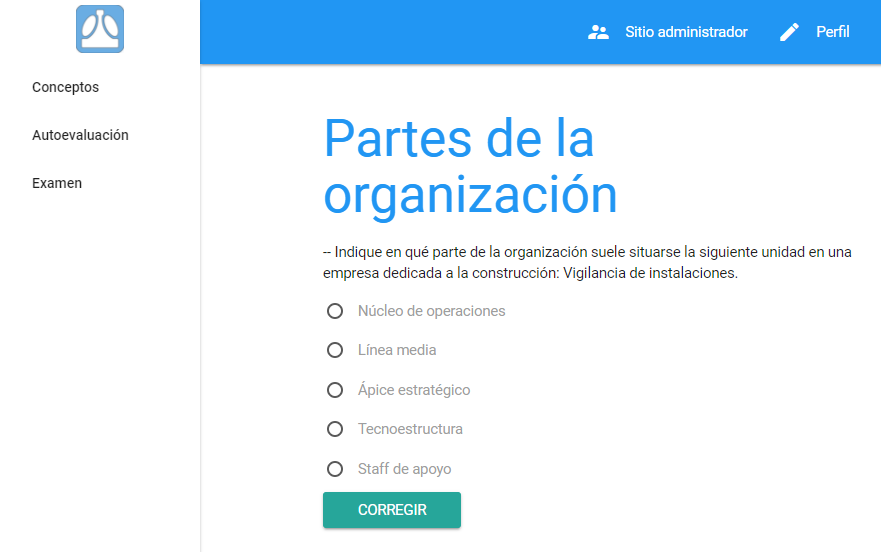
\includegraphics[width=0.7\textwidth]{../images/manual/pregunta_opm.png}
    \caption{Pregunta de opción múltiple}
    \label{fig:man_pregunta_opm}
\end{figure}


\bigskip
Una vez seleccionamos corregir, el sistema nos muestra la corrección de la actividad en la siguiente pantalla: 


\begin{figure}[!H]
 	\centering
 	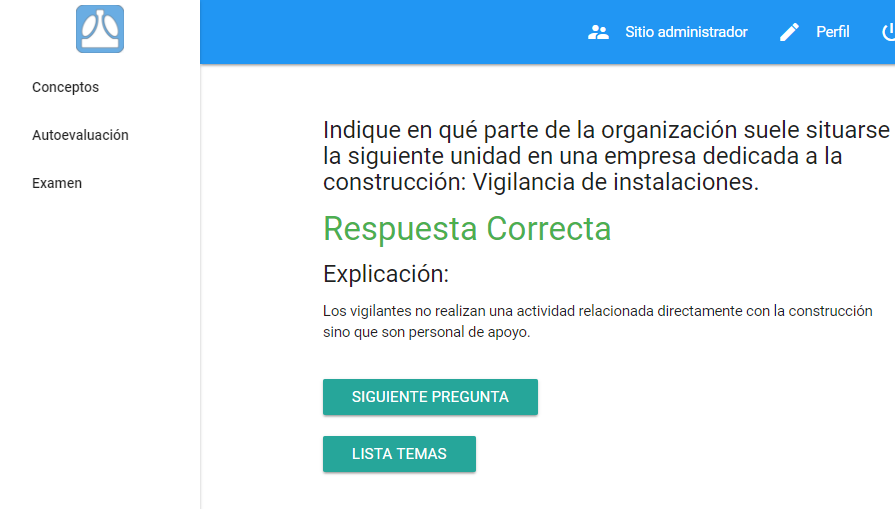
\includegraphics[width=0.7\textwidth]{../images/manual/pregunta_opm_respuesta.png}
    \caption{Corrección de la pregunta de opción múltiple.}
    \label{fig:man_pregunta_opm_respuesta}
\end{figure}







\newpage
\subsection{Examen}
\bigskip
Similar a la sección de ``Autoevaluación'', al entrar en esta sección el sistema muestra la lista de tipos de exámenes que podemos realizar. Al seleccionar alguno de ellos, entramos en el examen. Los exámenes son una recopilación aleatoria de preguntas de todos los temas de la asignatura. Imagen 
\ref{fig:man_examen_opm}.




\begin{figure}[!H]
 	\centering
 	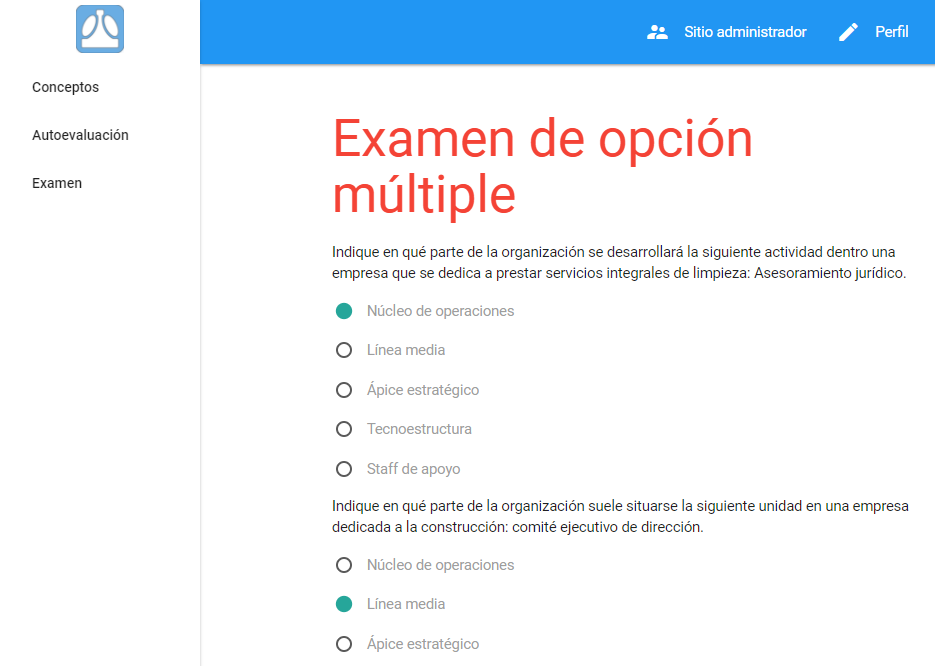
\includegraphics[width=0.7\textwidth]{../images/manual/examen_opm.png}
    \caption{Examen de preguntas de opción múltiple.}
    \label{fig:man_examen_opm}
\end{figure}



\begin{figure}[!H]
 	\centering
 	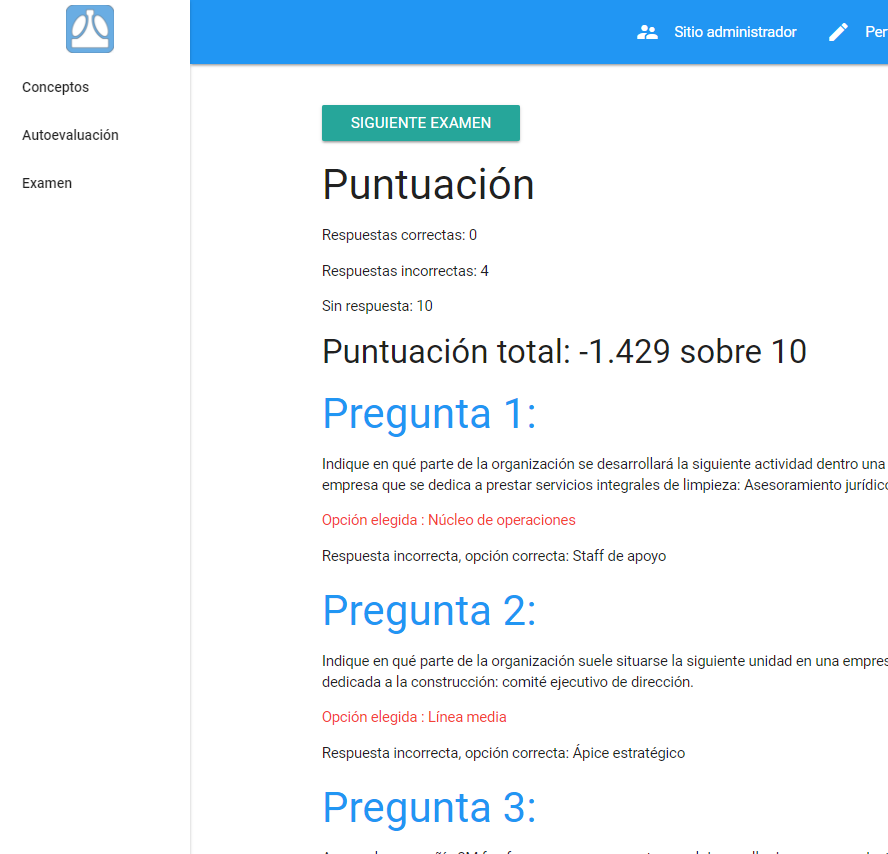
\includegraphics[width=0.7\textwidth]{../images/manual/examen_opm_respuesta.png}
    \caption{Corrección de examen.}
    \label{fig:man_examen_opm_respuesta}
\end{figure}



\subsection{Perfil}
\bigskip
En la barra de menú superior, tenemos la opción del perfil de usuario. Aquí encontramos las estadísticas del usuario y sus datos. Existe una pequeña diferencia entre los dos tipos de usuarios (profesor y alumno) y es que en la vista del usuario profesor se muestra una nueva sección para poder consultar los perfiles de sus alumnos y consultar sus estadísticas.
 Imagen \ref{fig:man_perfil_profesor}.


\begin{figure}[!H]
 	\centering
 	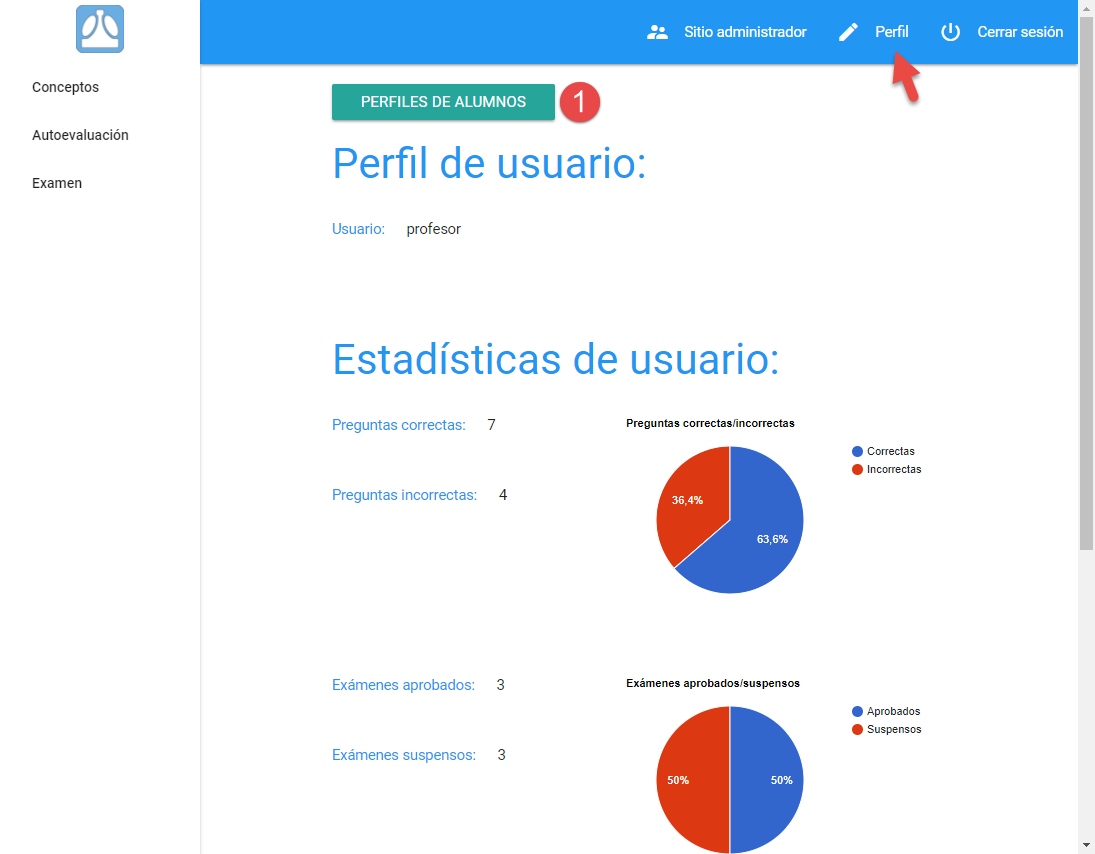
\includegraphics[width=0.8\textwidth]{../images/manual/perfil_profesor.png}
    \caption{Perfil del usuario profesor.}
    \label{fig:man_perfil_profesor}
\end{figure}

\bigskip
El perfil del usuario alumno es igual a excepción de esta funcionalidad.


\subsection{Sitio administrador}

\bigskip
El sitio administrador sólo está disponible para el usuario profesor y en él podrá actualizar la base de datos de la aplicación dividida en 3 secciones: 

\begin{itemize}
    \item Actualizar conceptos
    \item Actualizar preguntas verdadero falso.
    \item Actualizar preguntas de opción múltiple.
 \end{itemize}

 Podemos ver la pantalla en la imagen \ref{fig:man_administrador}.


\begin{figure}[!H]
 	\centering
 	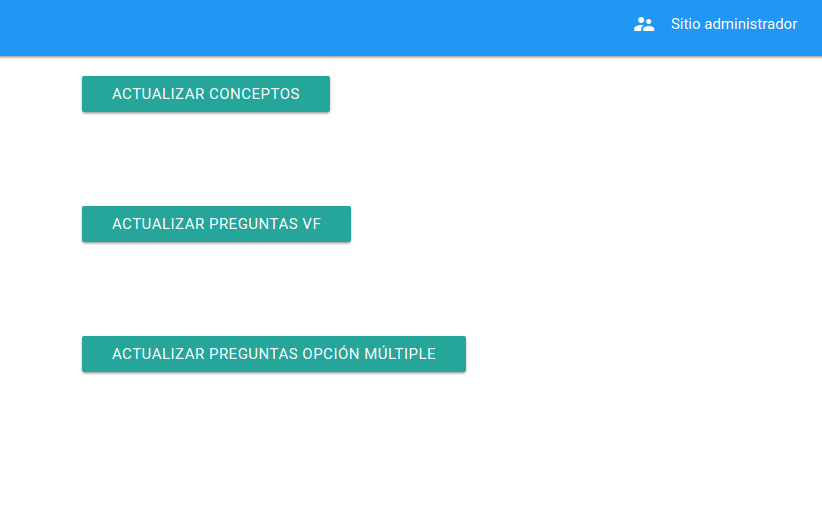
\includegraphics[width=0.8\textwidth]{../images/manual/administrador.png}
    \caption{Sitio de administración.}
    \label{fig:man_administrador}
\end{figure}